
%%%%%%%%%%%%%%%%%%
%                %
% Introduction   %
%                %
\chapter{Introduction}
\label{cp:intro}

%\begin{highlight}
%    \begin{st}
%        General structure with just some dummy text.
%    \end{st} 
%\end{highlight}

\lettrine{M}{obile robots} are a class of robots with the ability to move through the environment~\citep{corke2017robotics}. Most of these robots are power-demanding devices constrained by battery limitations. Although such limitations are a common challenge in many areas, they are critical in mobile robots' design and development. They influence the level of autonomy~\citep{seewald2020mechanical}, which in turn is expected to increase in the foreseeable future~\citep{fisher2013verifying}.

To move, mobile robots combine different components which sense and interact with the surrounding environment~\citep{mei2006deployment}. The analysis and interpretation of the data originating from these components often rely on high-level decisions. These are usually implemented on energy-demanding heterogeneous computing hardware. Planning an energy-aware path with a power-saving scheduling policy on such hardware is an underrepresented topic in the literature. Many past approaches focus almost exclusively on one of these topics. Some generate an energy-optimized path, despite the computations energy almost equaling the motion energy of some instances of low-energy mobile robots~\citep{sudhakar2020balancing}. Moreover, due to the recent advancements in the computational capabilities of heterogeneous computing hardware, such as the introduction of powerful portable GPUs\findex{GPU}~\citep{rizvi2017general}, the use of computations is on the rise~\citep{abramov2012real,satria2016real,jaramillo2019visual}. Others provide a power-saving scheduling policy. Yet, moving a mobile robot requires considerable energy expenditure over mere computations~\citep{mei2004energy,mei2005case}.

In this work, we focus on dynamic energy planning. We generate both an energy-aware plan of the path and a power-saving schedule of the computations. We plan these two aspects simultaneously, exploring their tradeoffs. We demonstrate the approach both in simulation and empirically, and we focus on aerial mobile robots. Although these systems share with the broader class of mobile robots stringent battery limitations, handling the battery in flight introduces additional complications. It is generally required landing to replace or recharge the battery~\citep{zamanakos2020energy}. Aerial robots are thus an ideal instance of energy-constrained systems that would benefit from a dynamic energy planning technique. In the remainder of this work, we thus focus our analysis on aerial robots.

There are many autonomous use cases involving aerial robots, such as precision agriculture, search and rescue, payload delivery, transportation, and many others. To formulate a mobile robot planning problem later in \fref{cp:pb}{Chapter}, we focus on precision agriculture and progressively build dynamic planning of a fixed-wing aerial robot flying over an agricultural field with little human input.

\begin{figure}[t]
  \centering
  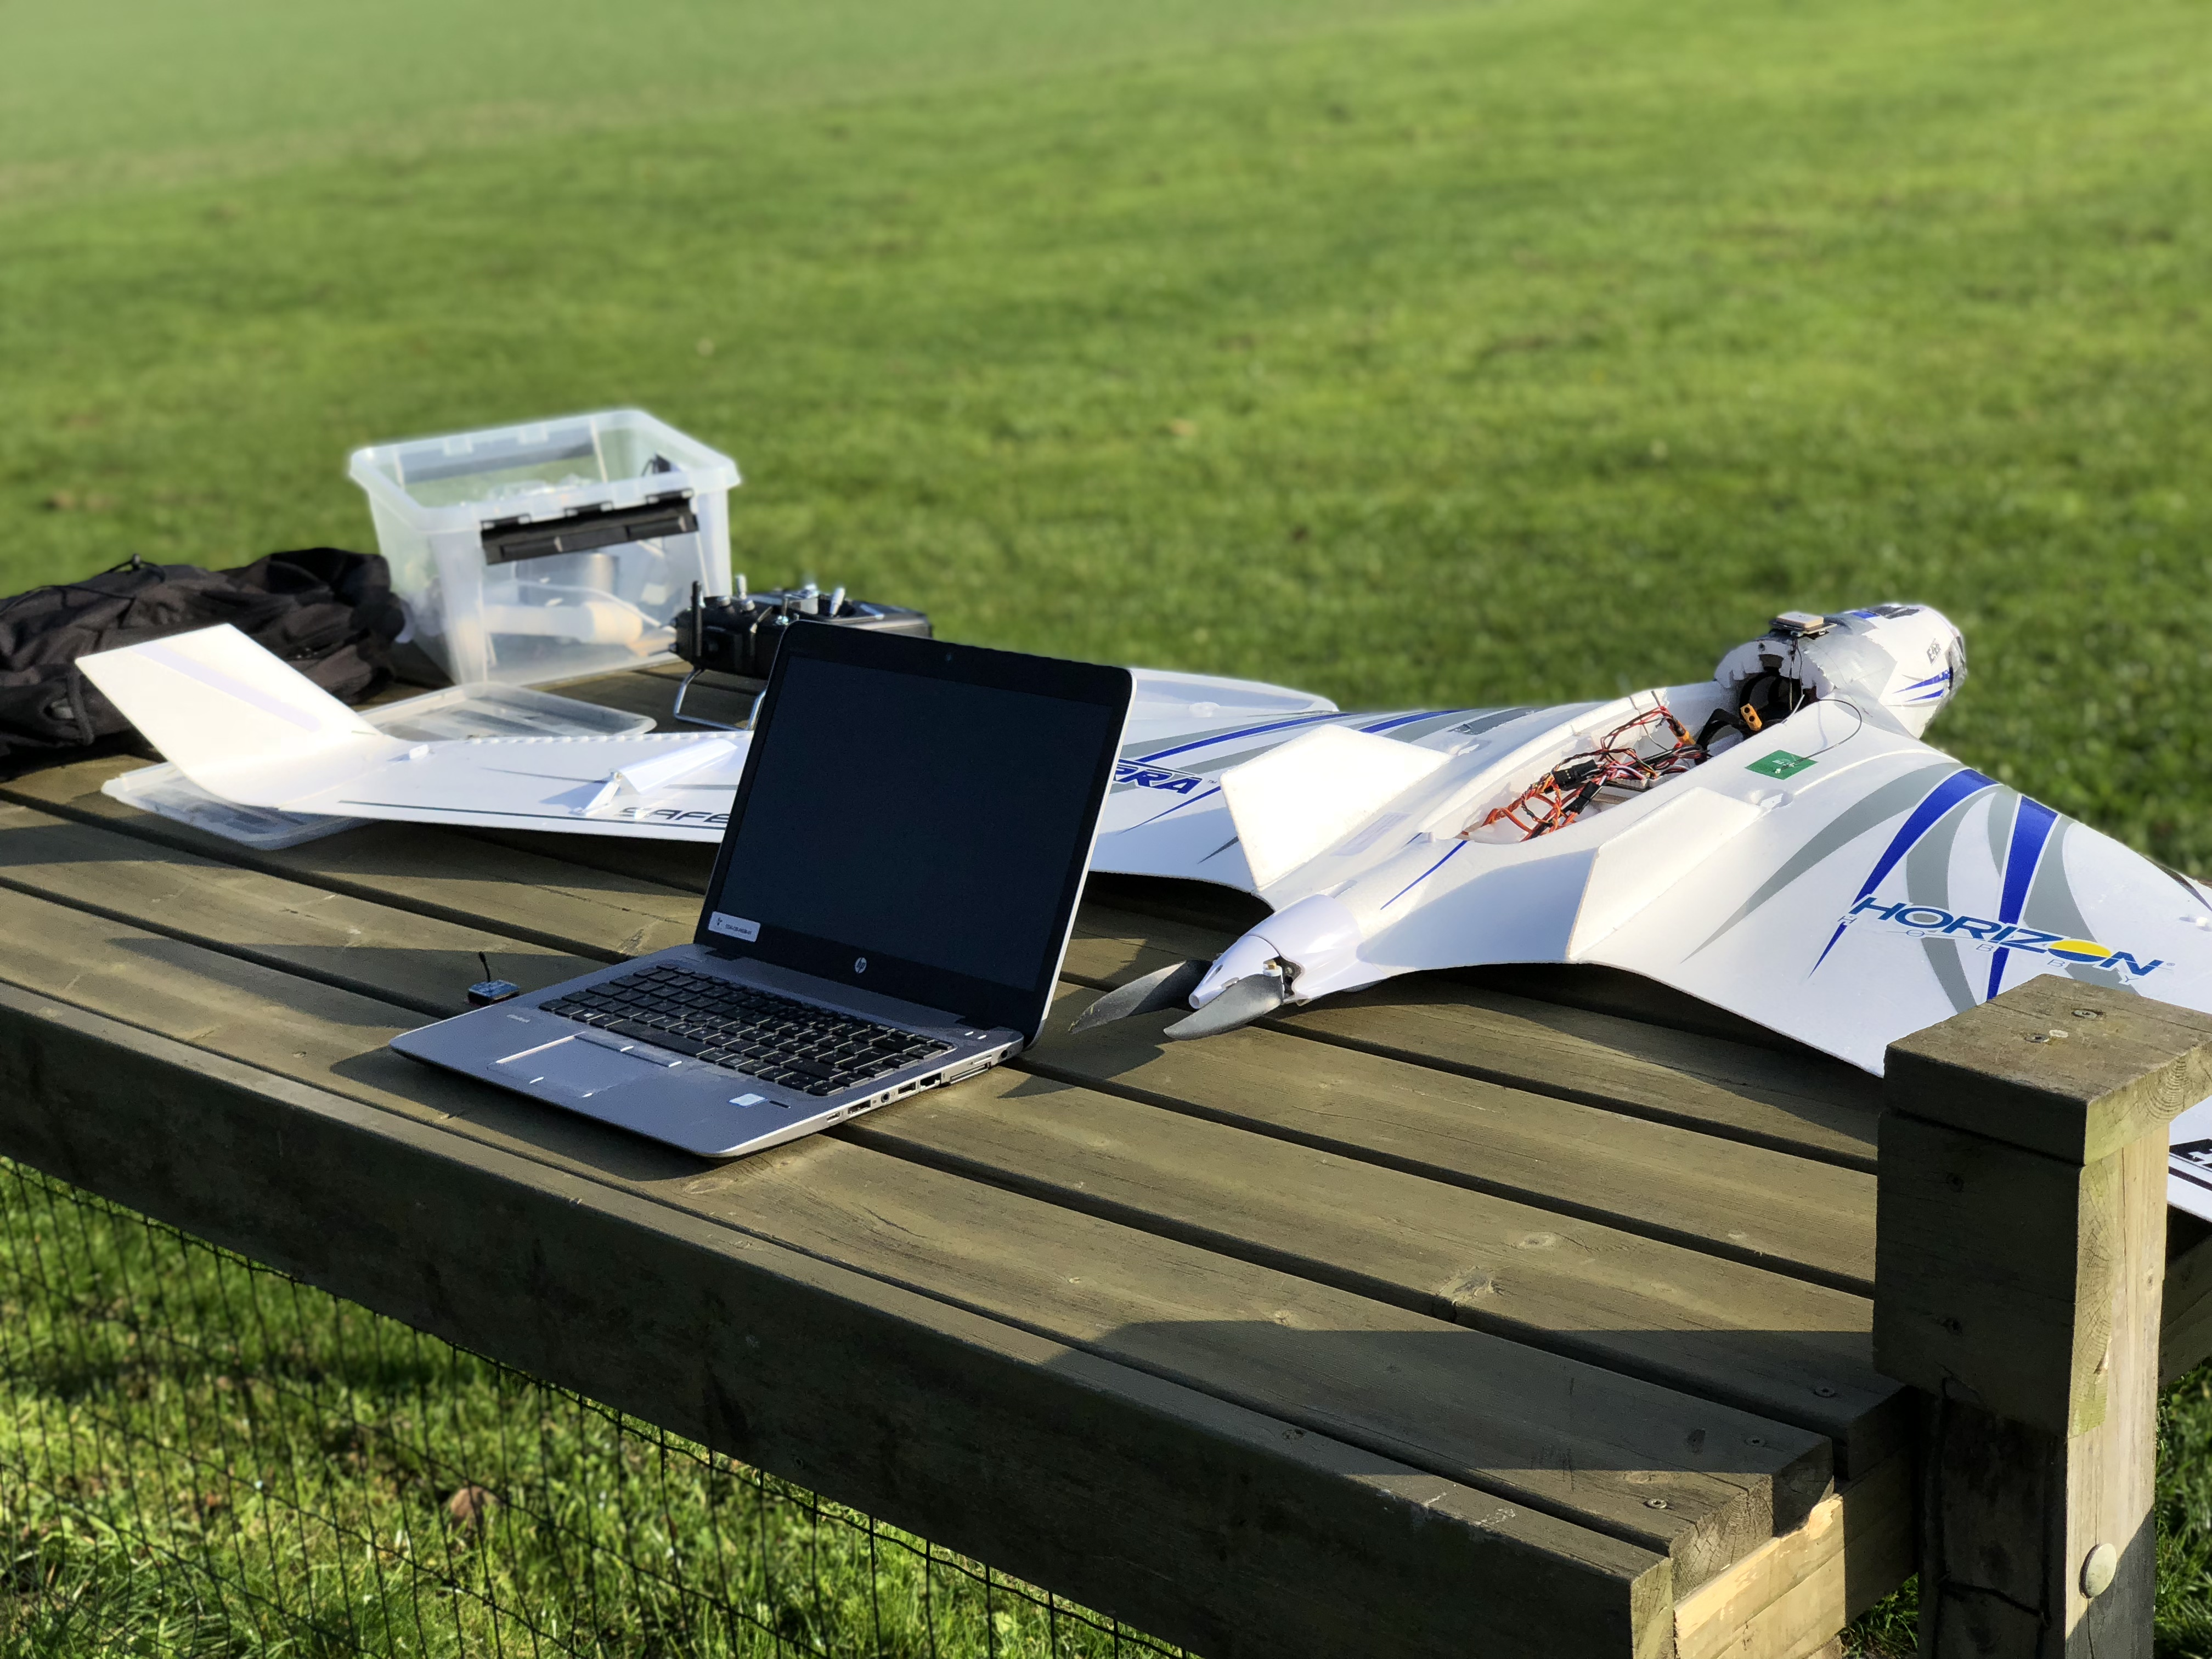
\includegraphics[width=.7\textwidth]{pictures/photo}
  \caption[Opterra fixed-wing aerial robot]{Opterra fixed-wing aerial robot employed for precision agriculture {\scriptsize(photo credit: Amit Ferencz Appel)}.}   
  \label{fig:opterra}
\end{figure}

We investigate different physical aerial robotics platforms in this work but we focus most on the Opterra fixed-wing aerial robot\findex{Opterra fixed-wing aerial robot}~\citep{opterra} adapted for precision agriculture. Precision agriculture\findex{precision agriculture} is often put into practice~\citep{hajjaj2014review} with ground mobile robots used for harvesting~\citep{qingchun2012study,dong2011development, de2011design, aljanobi2010setup, li2008analysis, edan2000robotic}, and unmanned aerial vehicles (\Gls{acr:uav}s) for preventing damage and ensuring better crop quality~\citep{puri2017agriculture, daponte2019review}. The aerial robot is shown in \fref{fig:opterra}{Figure}.

In the remainder of the chapter and before we introduce the problem in \fref{cp:pb}{Chapter}, we briefly investigate the evolution of the field of aerial robotics in the next section. We then analyze the main aerial robots available today, and how they apply to dynamic energy planning in \fref{sec:aerial-robo-types}{Section}. We then provide some further motivation for our planning in \fref{sec:motivation}{Section} and the outline of the approach in \fref{sec:outline}{Section}. Finally, we provide the structure of the remaining chapters in \fref{sec:structure}{Section}.

This chapter connects to the remainder of this work as follows. Here we introduce and motivate the dynamic energy planning for autonomous aerial robots. We formalize the planning problem in \fref{cp:pb}{Chapter}. We describe the derivation of a proper energy model to predict the future energy consumption of the planning problem in \fref{cp:model}{Chapter}. We estimate some coefficients of the model using robust estimation techniques in \fref{cp:est}{Chapter}. We implement an optimal configuration of the path and computations using data-driven control\findex{data-driven control} and other modern optimal control techniques in \fref{cp:opt}{Chapter}. We use such configuration for guidance and scheduling of the aerial robot in \fref{cp:gd}{Chapter}. The guidance moves physically the robot; the scheduling defines the granularity of the tasks being executed in flight. Moreover, we discuss previous approaches to solve the dynamic planning problem in \fref{cp:soa}{Chapter}. 


%%%%%%%%%%%%%%%%%%%%%%%%%%%%%%%%%%%%%%%%%%%
\section{From UAVs to Modern Aerial Robots}

Modern aerial robots are a valuable tool in robotic research and aerospace. They are found with different names in the literature. These include unmanned aerial vehicles\findex{unmanned aerial vehicles} (\Gls{acr:uav}s)\footnote{The term unmanned is sometimes replaced by uninhabited}, unmanned aerial systems\findex{unmanned aerial systems} (\Gls{acr:uas}s), flying robots, or drones. Usually, we refer to drones, \Gls{acr:uav}s, and \Gls{acr:uas}s when these systems are semi-autonomous, operated from the ground. \Gls{acr:uas} often denotes the entire infrastructure of unmanned flight in the aerospace jargon. Aerial or flying robots, on the other hand, have advanced levels of autonomy~\citep{siciliano2016springer}. Nevertheless, all these systems have basic autonomous features such as position and altitude holding and leveling. The position holding is usually implemented using global navigation satellite system\findex{global navigation satellite system} (\Gls{acr:gnss}), altitude holding using a barometer\findex{barometer}, and leveling using inertial measurement unit\findex{inertial measurement unit} (\Gls{acr:imu}).

\begin{figure}[t]
  \centering
  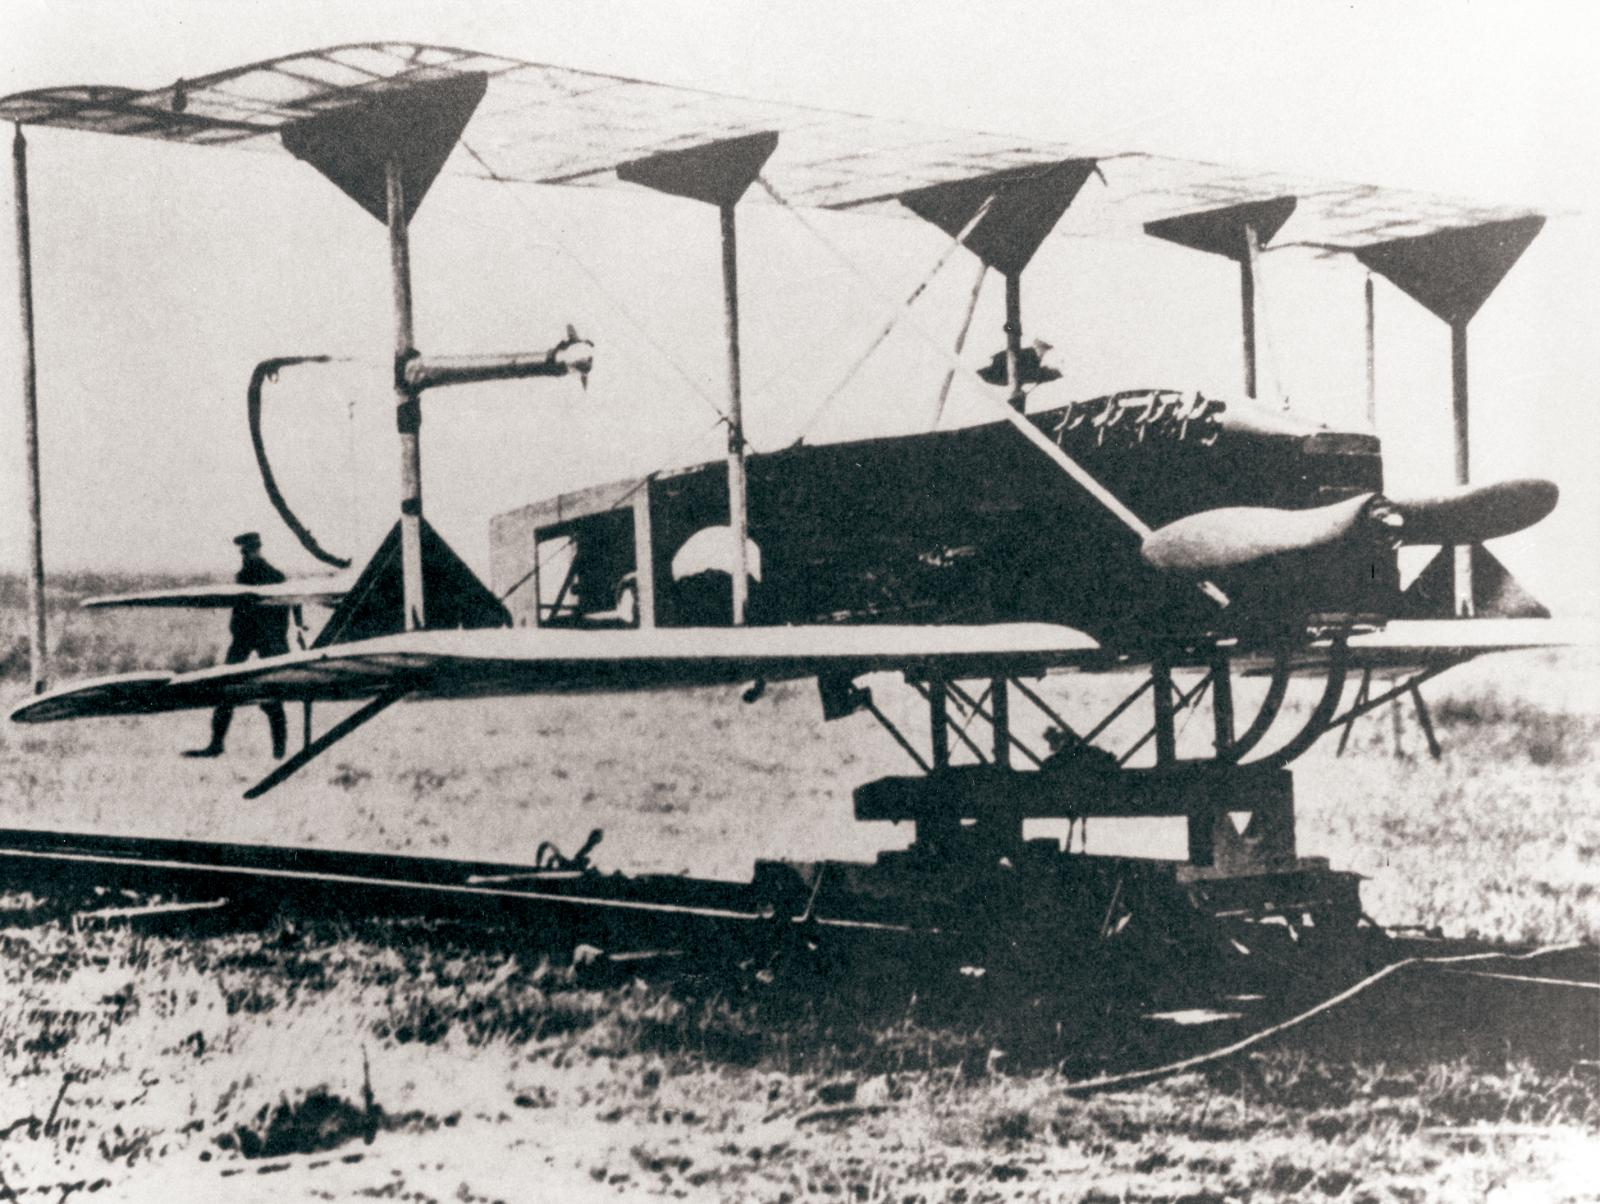
\includegraphics[width=.7\textwidth]{pictures/HA-NH-JA-19_1}
  \caption[Hewitt-Sperry Automatic Airplane, first unmanned flying machine]{The Hewitt-Sperry Automatic Airplane, also denominated ``flying bomb'', was developed in WWI and represents the first instance of a \Gls{acr:uav} {\scriptsize(photo credit: United States Naval Institute)}.}   
  \label{fig:hewitt-sperry}
\end{figure}

The origin of the field of aerial robotics, which deals with the design and development of aerial robots, dates back to the first guided missiles: unmanned (or uninhabited) flight has more than a century of developments~\citep{siciliano2016springer}. Hewitt-Sperry Automatic Airplane\findex{Hewitt-Sperry automatic airplane}, also denominated ``flying bomb'', developed in 1917 during World War I\findex{World War I} (WWI)~\citep{keane2013brief,valavanis2015handbook} is often referred to as the first unmanned flying machine. It is shown in \fref{fig:hewitt-sperry}{Figure}. It has been developed 14 years after the first heavier-than-air flight in history, demonstrated on December 17, 1903, with the Wright Flyer I by Wilbur and Orville Wright\findex{Wright brother} (or the Wright brothers). The Hewitt-Sperry Automatic Airplane used a gyroscope\findex{gyroscope} similarly to modern aerial robots. The device, invented by Elmer Sperry~\citep{keane2013brief}, was mechanically connected to the control surfaces and successfully implemented a control feedback loop~\citep{siciliano2016springer}.

In the early days, the first flying machines were referred to as remotely piloted vehicles\findex{remotely piloted vehicles} (\Gls{acr:rpv}s)~\citep{anderson2005introduction}. Many instances from WWI on of these vehicles were designed for military purposes. In the 1950s, United States used a remotely controlled vehicle, the Ryan Firebee\findex{Ryan Firebee}, for reconnaissance in Vietnam, and Israel was the first to use a \Gls{acr:rpv} in a combat situation~\citep{anderson2005introduction}. Other instances of these vehicles include the V-1 flying bomb~\findex{V-1 flying bomb} from 1944 (deployed by the unified armed forces of nazi Germany) and the Lockheed D-21~\findex{Lockheed D-21} from 1962 (deployed by the United States Air Force). Global positioning system\findex{global positioning system} (\Gls{acr:gps}) at the end of 1970 allowed some more recent remotely piloted vehicles to be used in surveillance. These systems were later integrated with cameras and other sensors~\citep{siciliano2016springer}, in what are the modern aerial robots.

In recent years, the unmanned flight has been applied in many civilian applications~\citep{gonzalez2017unmanned}. Modern aerial robots are increasingly used in remote sensing\findex{remote sensing}~\citep{noor2018remote,tang2015drone,milas2018drones}, surveillance\findex{surveillance}~\citep{paucar2018use,burkle2009collaborating}, meteorology\findex{meteorology}~\citep{schuyler2019using}, search and rescue\findex{search and rescue}~\citep{pensieri2020drones,karaca2018potential,cui2015drones,seguin2018unmanned}, precision agriculture~\citep{daponte2019review,puri2017agriculture}, transportation, and payload delivery\findex{payload delivery}~\citep{kellermann2020drones}. The former four categories fall into the area of reconnaissance, surveillance, and target acquisition\findex{reconnaissance, surveillance, and target acquisition} (\Gls{acr:rsta}) and do not require advanced autonomy. Precision agriculture, transportation, and payload delivery are often realized using to a greater or lesser extent some advanced levels of computational intelligence~\citep{siciliano2016springer}. Modern aerial robots are designed to handle unexplored terrain with little interaction as opposed to the past \Gls{acr:uav}s operated mainly by a human operator~\citep{siciliano2016springer}. Instances of modern aerial robots are expected to autonomously adapt and possibly interact in a broad variety of environmental conditions. 

\begin{figure}[t]
  \centering
  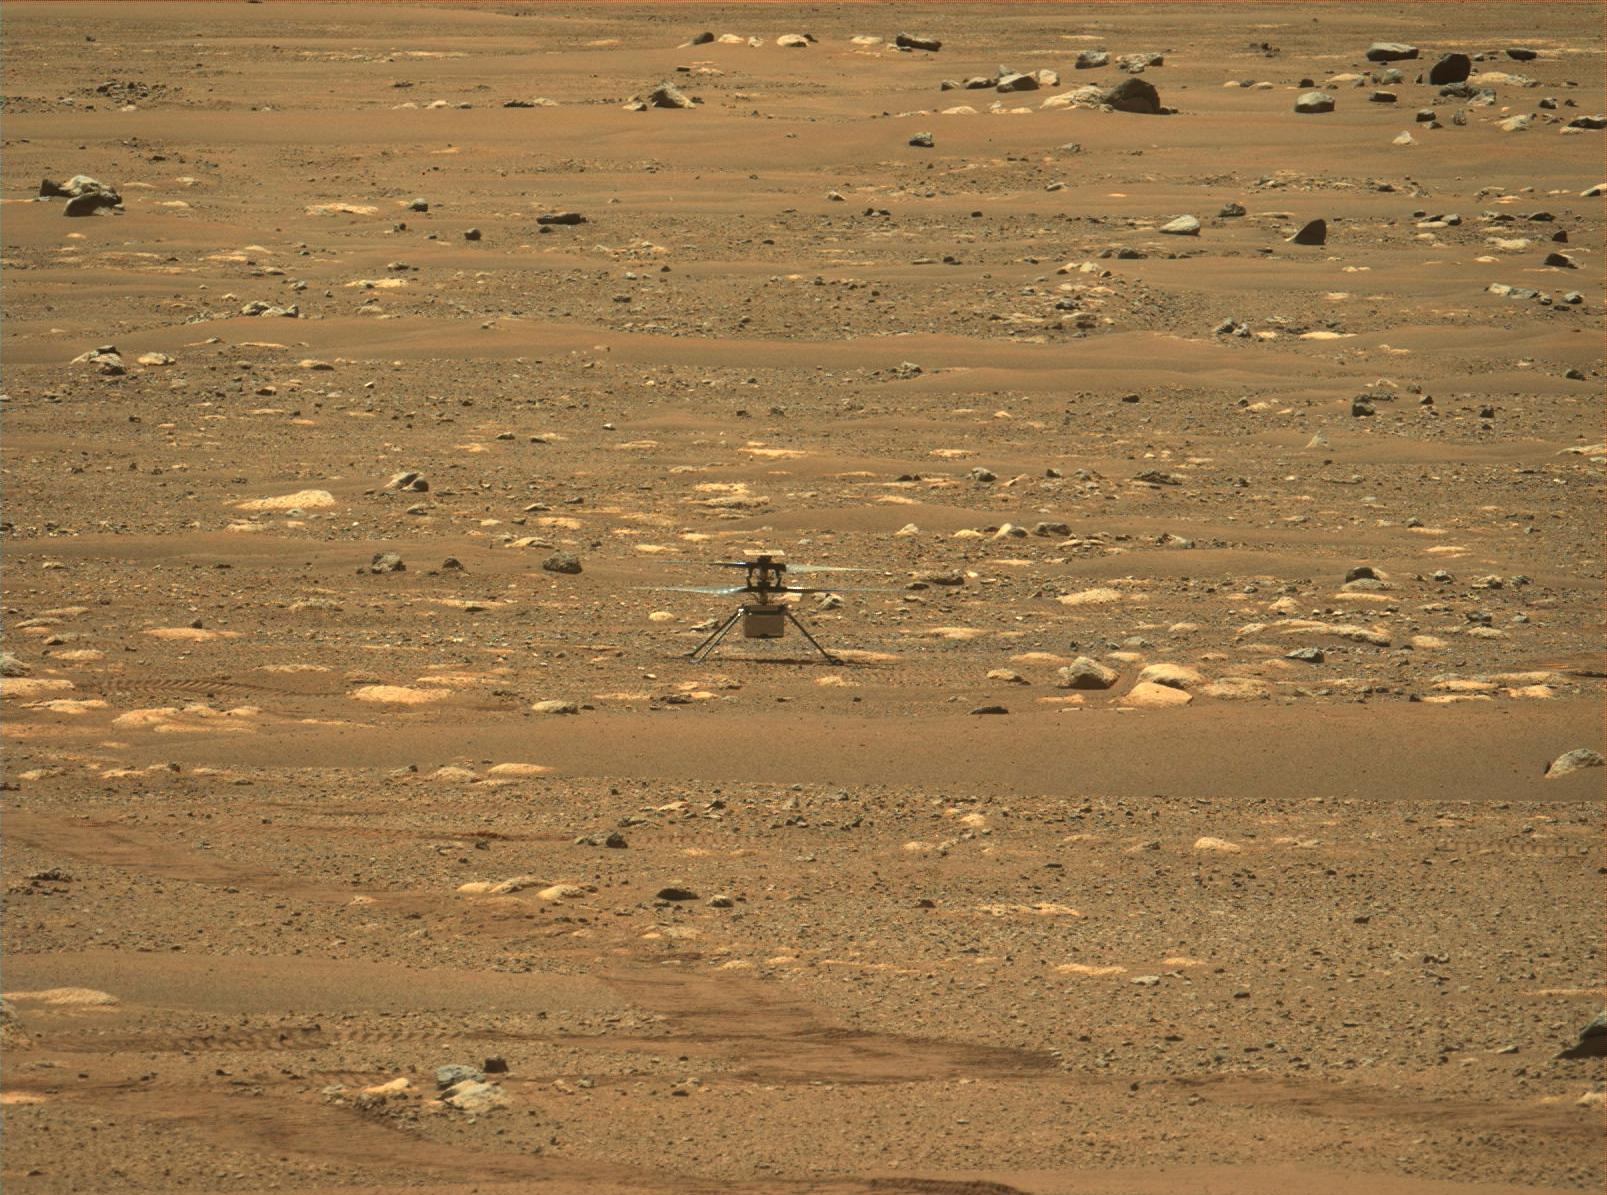
\includegraphics[width=.7\textwidth]{pictures/jpegPIA24550}
  \caption[NASA's Ingenuity Mars Helicopter]{NASA's Ingenuity Mars Helicopter. A rotary-wing coax aerial robot that achieved the first powered, controlled flight on another planet on April 19, 2021. The project is solely a demonstration of technology {\scriptsize(photo credit: NASA Jet Propulsion Laboratory)}.}   
  \label{fig:ingenuity}
\end{figure}

In summary, aerial robots have a relatively recent past. Some initial experiments of unmanned flights were performed shortly after the first heavier-than-air manned, powered flight. These initial experiments were mostly developed for military purposes, whereas modern aerial robots are used in a broad range of civil applications. Aerial robots are expected to grow significantly in numerous areas of robotics research ranging from agriculture to planetary exploration. For the latter, \fref{fig:ingenuity}{Figure} shows NASA's Ingenuity Mars Helicopter. A small coaxial aerial robot that performed the first powered, controlled flight on another planet on April 19, 2021. Aerial robots for planetary exploration are to be further deployed in future explorations endeavors, for instance, to study Saturn's moon Titan~\citep{voosen2019nasa}.

Finally, we conclude this section with a quote from~\citep{anderson2005introduction}: ``the Wright brothers worked so hard to put humans in the air in flying machines, a hundred years later some [...] are working hard to take them out of flying machines''.


%%%%%%%%%%%%%%%%%%%%%%%%%%%%%%%%%%%%%%%%%
\section{Common Classes of Aerial Robots}
\label{sec:aerial-robo-types}

Numerous different types of aerial robots have emerged ever since their first introduction. We briefly investigate the most studied classes in the robotics literature and relate them to the dynamic energy planning that we focus on in this work. The two most generic classes are heavier-than-air and lighter-than-air aerial robots. Heavier-than-air aerial robots\findex{heavier-than-air aerial robots} are divided into fixed- and rotary-wings~\citep{siciliano2016springer}, and some recent developments in bio-inspired robotics study flapping-wings~\citep{floreano2015science}\findex{flapping-wings}. 

Rotary-wing aerial robots\findex{rotary-wings} are highly maneuverable and can perform stationary vertical flight (commonly referred to as hovering\findex{hovering})~\citep{siciliano2016springer}. These systems can be classified into further categories, which include multirotors\findex{multirotors} (such as quadrotors\findex{quadrotors} or quadcopters\findex{quadcopters}, hexacopters\findex{hexacopters}, and octocopters\findex{octocopters}), conventional helicopters\findex{helicopters} (these have one main and one tail rotor), and a coax\findex{coax} (these have counter-rotating coaxial rotors)~\citep{corke2017robotics}. Some examples of quadrotors are DJI Mavic Mini in \sref{lab:mavic}, and DJI Phantom 4 in \sref{lab:phantom} in \fref{fig:plot10}{Figure}. In the same figure, DJI Agras T16 in \sref{lab:agras}, and DJI Matrice 600 in \sref{lab:matrice} are hexacopters.

Fixed-wing aerial robots\findex{fixed-wings} have wings to provide the lift, some control surfaces for maneuvering, and a propeller for forward thrust; a shared principle with a common passenger aircraft~\citep{corke2017robotics}. An example constitutes the Opterra adapted for precision agriculture in \fref{fig:opterra}{Figure}, Cumulus in \sref{lab:cumulus}, Ebee in \sref{lab:ebee}, and Penguin BE in \sref{lab:penguin}~\citep{haugen2016monitoring} in \fref{fig:plot10}{Figure}. Examples of flapping-wings are Delfly II in \sref{lab:delfly}~\citep{percin2012flow}, and Nano-Hummingbird in \sref{lab:nano} in \fref{fig:plot10}{Figure}. We discuss in detail heavier-than-air aerial robots in this work, as they are a common platform for robotics research. We focus on the dynamic forces which govern the flight of rotary- and fixed-wings aerial robots in \fref{cp:gd}{Chapter}.

Common instances of lighter-than-air aerial robots\findex{lighter-than-air aerial robots} are blimps\findex{blimps} (or non-rigid airships). They usually rely on a gas--such as helium enclosed in a protected envelope~\citep{burri2013design}--to generate the lifting force~\citep{fui2017recent}. An omnidirectional spherical blimp is shown in \fref{fig:skye-blimp}{Figure}. Blimps are similar to balloons but provide basic maneuverability, whereas, in a balloon, only the altitude can be controlled~\citep{colombatti2011lighter}.

\begin{figure}[t]
  \centering
  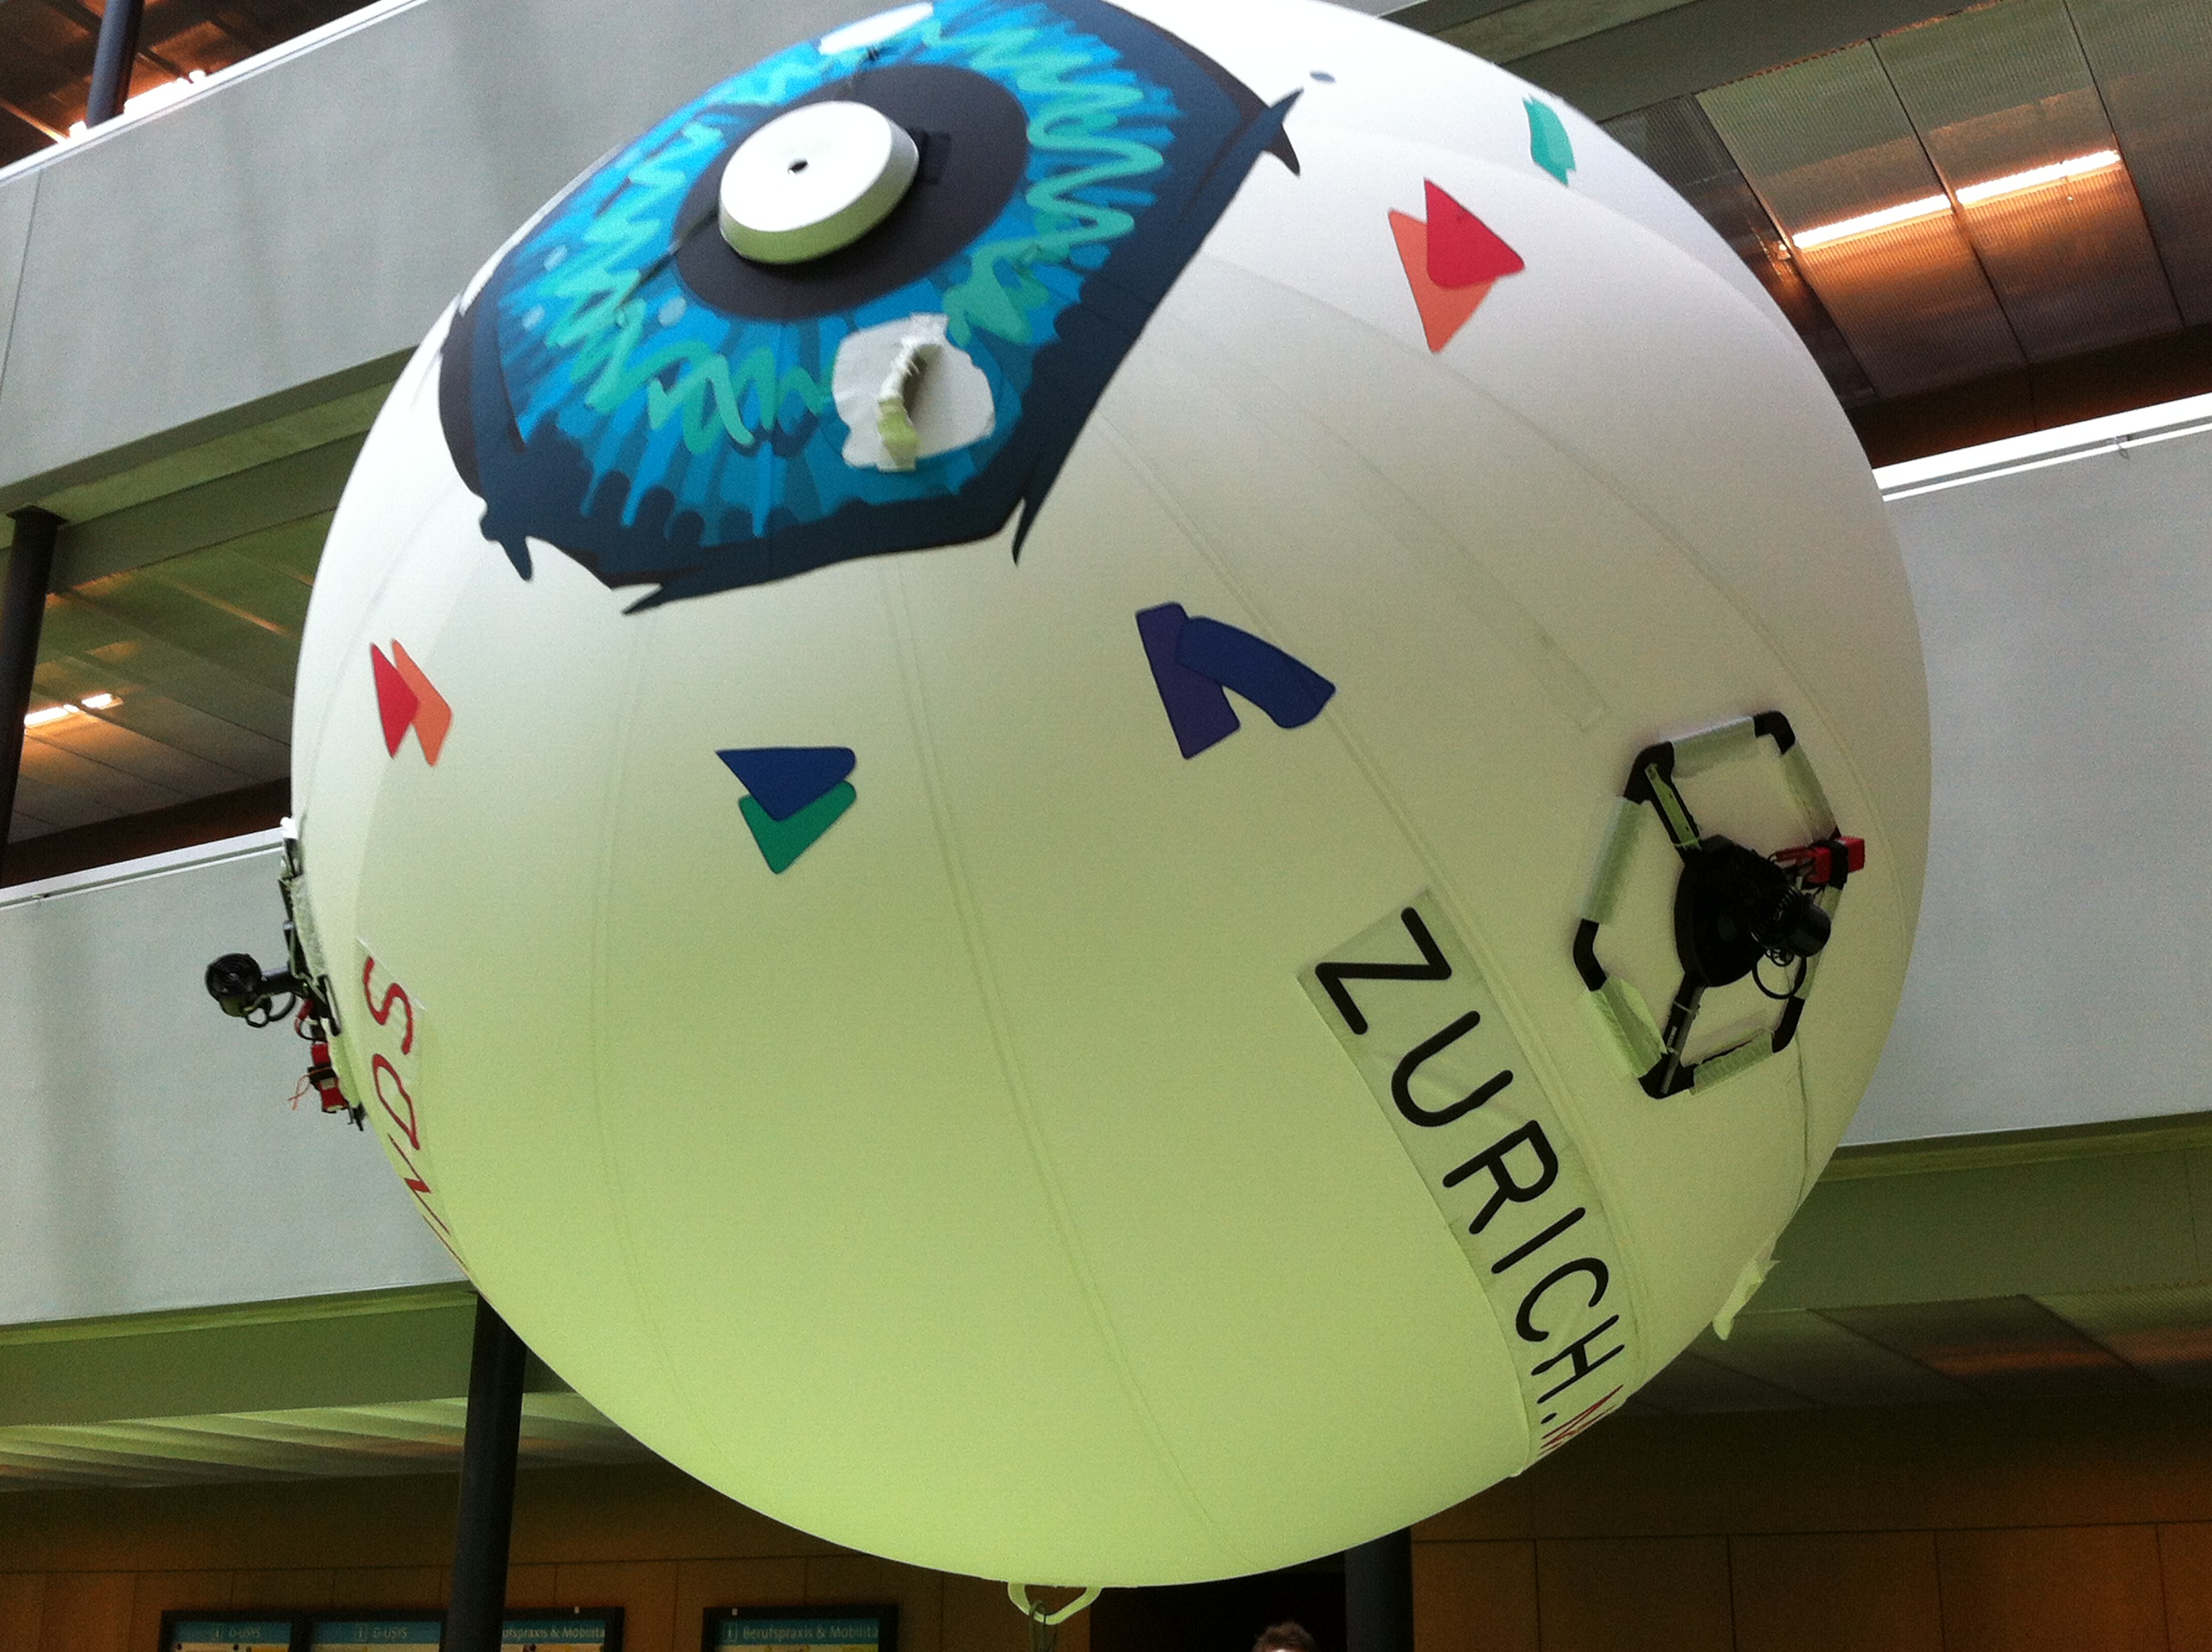
\includegraphics[width=.7\textwidth]{pictures/IMG_2612}
  \caption[Skye, an omnidirectional spherical blimp]{Skye, an omnidirectional spherical blimp developed by ETH Z\"urich for entertainment purposes. It has a camera system and combines the energy-efficient flight of a blimp with the characteristics of a quadrotor {\scriptsize(photo credit: ETH Z\"urich)}.}   
  \label{fig:skye-blimp}
\end{figure}

Some other classifications found in aerial robotics literature trade size and maneuverability and include classes as micro aerial vehicles (MAVs)\findex{micro aerial vehicles} or vertical take-off and landing (VTOLs)\findex{vertical take-off and landing} aerial robots. The former are aerial robots with all dimensions lower than 15 cm. The latter are aerial robots flying in a fixed-wing configuration except if taking-off and landing where they use thrust from rotors rather than lift from wings. 

Among the classes in this section, rotary-wings are the most maneuverable and lighter-than-air aerial robots are the least. These, however, have the highest flight time followed by fixed-wing aerial robots. Mixed configurations, such as VTOLs, fall into the intersection of rotary and fixed-wings for what concerns maneuverability and flight time~\citep{siciliano2016springer}. The energy requirements are critical for all aerial robots, but the difference of motion and computations energy (\Gls{acr:mace}) varies greatly. The energy--inversely proportional to flight time--is highest in rotary-wings and lowest in lighten-than-air aerial robots as shown later in \fref{fig:plot10}{Figure}. The dynamic energy planning approach thus relies on both power-saving task scheduling and energy-efficient path planning for the fixed-wings robots while relying almost exclusively on energy-efficient path planning for rotary-wing aerial robots. In the former \Gls{acr:mace} is close to zero, in the latter is usually high except in energy optimized designs such as some rotary-wing MAVs. Hypothetically, in lighter-than-air aerial robots, \Gls{acr:mace} might be negative; the energy planning approach would rely heavily on power-saving task scheduling.


%%%%%%%%%%%%%%%%%%%%
\section{Motivation}
\label{sec:motivation}

\begin{figure}[t!]
  \centering
  \footnotesize\fontfamily{phv}\selectfont
  
\definecolor{cF5F5F5}{RGB}{245,245,245}
\definecolor{cE4E4E4}{RGB}{218,218,218}
\definecolor{cFFFFFF}{RGB}{255,255,255}


\def \globalscale {1.000000}
\begin{tikzpicture}[y=0.80pt, x=0.80pt, yscale=-\globalscale, xscale=\globalscale, inner sep=0pt, outer sep=0pt]
\path[fill=cF5F5F5,line join=round,line width=0.160pt] (49.4778,304.7930) .. controls (49.4778,304.7930) and (59.8838,312.4890) .. (61.2031,312.8170) .. controls (70.4387,315.1130) and (100.8800,325.1290) .. (113.9110,320.3850) .. controls (113.9110,320.3850) and (128.5000,319.7570) .. (145.0340,312.7870) .. controls (161.5680,305.8160) and (145.5200,259.4940) .. (145.5200,259.4940) .. controls (145.5200,259.4940) and (142.1620,253.0560) .. (134.1470,241.3320) .. controls (117.8560,217.5040) and (93.7304,210.8650) .. (93.7304,210.8650) .. controls (93.7304,210.8650) and (63.8068,187.8810) .. (25.8309,187.8090) .. controls (25.8308,187.8090) and (-22.5721,198.7600) .. (27.1148,283.8080) -- (49.4778,304.7930) -- cycle;



\path[fill=cE4E4E4,line join=round,line width=0.160pt] (127.5850,194.5280) .. controls (127.5850,194.5280) and (134.1470,175.0990) .. (158.4610,168.6670) .. controls (182.7760,162.2360) and (231.4050,165.3730) .. (280.0340,151.6470) .. controls (328.6630,137.9210) and (369.0490,168.6670) .. (369.0490,168.6670) .. controls (369.0490,168.6670) and (406.9790,216.5900) .. (336.4670,259.4940) .. controls (265.9550,302.3970) and (189.5610,259.9450) .. (182.7760,254.0000) .. controls (175.9910,248.0540) and (138.0740,250.1440) .. (129.7840,235.1790) .. controls (121.4930,220.2140) and (121.4250,207.4960) .. (127.5850,194.5280) -- cycle;



\path[fill=foo,line join=round,line width=0.160pt] (169.3250,153.3220) .. controls (169.3250,153.3220) and (214.3850,166.4820) .. (231.4050,160.2860) .. controls (231.4050,160.2860) and (248.7700,157.3510) .. (265.3040,150.3810) .. controls (281.8380,143.4110) and (280.0340,102.4370) .. (280.0340,102.4370) .. controls (280.0340,102.4370) and (278.7420,90.4098) .. (280.0340,76.2665) .. controls (282.4490,49.8338) and (244.5430,30.6534) .. (244.5430,30.6534) .. controls (244.5430,30.6534) and (236.2680,14.3982) .. (134.1470,38.7128) .. controls (134.1470,38.7128) and (106.5590,38.7128) .. (123.0930,135.9710) .. controls (123.0930,135.9710) and (144.3610,149.3270) .. (149.3680,151.1110) .. controls (154.3750,152.8940) and (169.0830,153.1350) .. (169.3250,153.3220) -- cycle;

\path[cm={{1.0,0.0,0.0,1.0,(0,0)}}] (0.0000,0.0000) node[below right] () {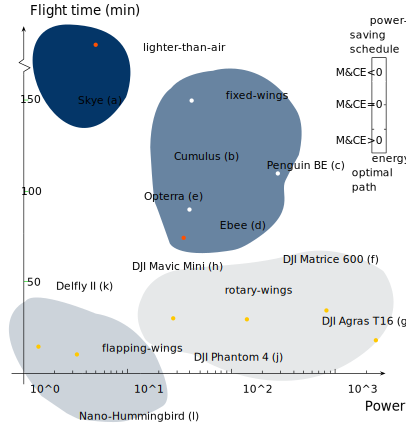
\includegraphics[width=4.25in]{figures/source/plot10}};

\path[fill=foo,line join=round,line width=0.160pt] (319.5490,240.6600) .. controls (320.7430,240.6600) and (321.7110,241.6280) .. (321.7110,242.8220) .. controls (321.7110,244.0160) and (320.7430,244.9840) .. (319.5490,244.9840) .. controls (318.3550,244.9840) and (317.3870,244.0160) .. (317.3870,242.8220) .. controls (317.3870,241.6280) and (318.3550,240.6600) .. (319.5490,240.6600) -- cycle;



\path[fill=foo,line join=round,line width=0.160pt] (269.0760,214.8400) .. controls (270.2700,214.8400) and (271.2380,215.8080) .. (271.2380,217.0020) .. controls (271.2380,218.1960) and (270.2700,219.1640) .. (269.0760,219.1640) .. controls (267.8820,219.1640) and (266.9140,218.1960) .. (266.9140,217.0020) .. controls (266.9140,215.8080) and (267.8820,214.8400) .. (269.0760,214.8400) -- cycle;



\path[fill=foo,line join=round,line width=0.160pt] (208.4930,224.7000) .. controls (209.6870,224.7000) and (210.6550,225.6680) .. (210.6550,226.8620) .. controls (210.6550,228.0560) and (209.6870,229.0240) .. (208.4930,229.0240) .. controls (207.2990,229.0240) and (206.3310,228.0560) .. (206.3310,226.8620) .. controls (206.3310,225.6680) and (207.2990,224.7000) .. (208.4930,224.7000) -- cycle;



\path[fill=foo,line join=round,line width=0.160pt] (201.7350,224.7000) .. controls (202.9290,224.7000) and (203.8970,225.6680) .. (203.8970,226.8620) .. controls (203.8970,228.0560) and (202.9290,229.0240) .. (201.7350,229.0240) .. controls (200.5410,229.0240) and (199.5730,228.0560) .. (199.5730,226.8620) .. controls (199.5730,225.6680) and (200.5410,224.7000) .. (201.7350,224.7000) -- cycle;



\path[fill=cFFFFFF,line join=round,line width=0.160pt] (231.4380,85.7318) .. controls (232.6320,85.7318) and (233.6000,86.6998) .. (233.6000,87.8938) .. controls (233.6000,89.0879) and (232.6320,90.0560) .. (231.4380,90.0560) .. controls (230.2440,90.0560) and (229.2760,89.0879) .. (229.2760,87.8938) .. controls (229.2760,86.6998) and (230.2440,85.7318) .. (231.4380,85.7318) -- cycle;



\path[fill=cFFFFFF,line join=round,line width=0.160pt] (196.7440,73.3687) .. controls (197.9380,73.3687) and (198.9060,74.3367) .. (198.9060,75.5307) .. controls (198.9060,76.7248) and (197.9380,77.6928) .. (196.7440,77.6928) .. controls (195.5500,77.6928) and (194.5820,76.7248) .. (194.5820,75.5307) .. controls (194.5820,74.3367) and (195.5500,73.3687) .. (196.7440,73.3687) -- cycle;



\path[fill=cFFFFFF,line join=round,line width=0.160pt] (195.2150,96.1679) .. controls (196.4090,96.1679) and (197.3770,97.1359) .. (197.3770,98.3300) .. controls (197.3770,99.5240) and (196.4090,100.4920) .. (195.2150,100.4920) .. controls (194.0210,100.4920) and (193.0530,99.5240) .. (193.0530,98.3300) .. controls (193.0530,97.1359) and (194.0210,96.1679) .. (195.2150,96.1679) -- cycle;



\path[fill=cFFFFFF,line join=round,line width=0.160pt] (192.0210,91.8550) .. controls (193.2150,91.8550) and (194.1830,92.8230) .. (194.1830,94.0171) .. controls (194.1830,95.2111) and (193.2150,96.1791) .. (192.0210,96.1791) .. controls (190.8270,96.1791) and (189.8590,95.2111) .. (189.8590,94.0171) .. controls (189.8590,92.8230) and (190.8270,91.8550) .. (192.0210,91.8550) -- cycle;



\path[fill=foo,line join=round,line width=0.160pt] (77.3763,248.8450) .. controls (78.5704,248.8450) and (79.5384,249.8130) .. (79.5384,251.0070) .. controls (79.5384,252.2010) and (78.5704,253.1690) .. (77.3763,253.1690) .. controls (76.1823,253.1690) and (75.2143,252.2010) .. (75.2143,251.0070) .. controls (75.2143,249.8130) and (76.1823,248.8450) .. (77.3763,248.8450) -- cycle;



\path[fill=foo,line join=round,line width=0.160pt] (72.8985,245.0460) .. controls (74.0925,245.0460) and (75.0605,246.0140) .. (75.0605,247.2080) .. controls (75.0605,248.4020) and (74.0925,249.3700) .. (72.8985,249.3700) .. controls (71.7044,249.3700) and (70.7364,248.4020) .. (70.7364,247.2080) .. controls (70.7364,246.0140) and (71.7044,245.0460) .. (72.8985,245.0460) -- cycle;



\path[fill=foo,line join=round,line width=0.160pt] (19.1786,12.9659) .. controls (20.3727,12.9659) and (21.3407,13.9339) .. (21.3407,15.1280) .. controls (21.3407,16.3221) and (20.3727,17.2901) .. (19.1786,17.2901) .. controls (17.9845,17.2901) and (17.0165,16.3221) .. (17.0165,15.1280) .. controls (17.0165,13.9339) and (17.9845,12.9659) .. (19.1786,12.9659) -- cycle;



\path[fill=black,line join=round,line width=0.160pt] (320.5760,257.0980) -- (322.5520,259.3950) -- (320.5300,261.4530) -- (326.3250,259.3400) -- (320.5760,257.0980) -- cycle;



\path[fill=black,line join=round,line width=0.160pt] (180.7460,21.4106) -- (183.0180,19.4057) -- (185.1020,21.4014) -- (182.9160,15.6335) -- (180.7460,21.4106) -- cycle;



\path[draw=black,line join=round,line width=0.512pt] (41.4555,259.3320) -- (322.6080,259.3320);



\path[draw=black,line join=round,line width=0.512pt] (183.0230,266.9540) -- (183.0230,156.7750);



\path[draw=cFFFFFF,line join=round,line width=0.512pt] (183.0230,156.7750) -- (183.0230,28.8031);



\path[draw=black,line join=round,line width=0.512pt] (183.0230,28.8031) -- (183.0230,18.3373);



  \path[cm={{1.0,0.0,0.0,1.0,(240.0,39.0)}}] (0.0000,0.0000) node[above right] () {{\color{white}fix}ed-wings};



  \path[cm={{1.0,0.0,0.0,1.0,(138.0,11.0)}}] (0.0000,0.0000) node[above right] () {flight time};



  \path[cm={{1.0,0.0,0.0,1.0,(128.0,240.0)}}] (0.0000,0.0000) node[above right] () {\scriptsize DJI Mavic Mini  \textlabel{(h)}{lab:mavic}};



  \path[cm={{1.0,0.0,0.0,1.0,(303.0,239.0)}}] (0.0000,0.0000) node[above right] () {\scriptsize DJI Agras T16  \textlabel{(g)}{lab:agras}};



  \path[cm={{1.0,0.0,0.0,1.0,(223.0,213.0)}}] (0.0000,0.0000) node[above right] () {\scriptsize DJI Matrice 600  \textlabel{(f)}{lab:matrice}};



  \path[cm={{1.0,0.0,0.0,1.0,(209.0,276.0)}}] (0.0000,0.0000) node[above right] () {\scriptsize DJI Phantom 4  \textlabel{(j)}{lab:phantom}};



  \path[cm={{1.0,0.0,0.0,1.0,(138.0,86.0)}}] (0.0000,0.0000) node[above right] () {\scriptsize\color{white} Cumulus \textlabel{(b)}{lab:cumulus}};



  \path[cm={{1.0,0.0,0.0,1.0,(208.0,150.0)}}] (0.0000,0.0000) node[above right] () {\scriptsize\color{white} Opterra \textlabel{(e)}{lab:opterra}};



  \path[cm={{1.0,0.0,0.0,1.0,(143.0,144.0)}}] (0.0000,0.0000) node[above right] () {\scriptsize\color{white} Ebee \textlabel{(d)}{lab:ebee}};



  \path[cm={{1.0,0.0,0.0,1.0,(212.0,83.0)}}] (0.0000,0.0000) node[above right] () {\scriptsize\color{white} Penguin BE  \textlabel{(c)}{lab:penguin}};



  \path[cm={{1.0,0.0,0.0,1.0,(66.0,311.0)}}] (0.0000,0.0000) node[above right] () {\scriptsize Nano-Hummingbird  \textlabel{(l)}{lab:nano}};



  \path[cm={{1.0,0.0,0.0,1.0,(19.0,257.0)}}] (0.0000,0.0000) node[above right] () {\scriptsize Delfly II  \textlabel{(k)}{lab:delfly}};



  \path[cm={{1.0,0.0,0.0,1.0,(35.0,71.0)}}] (0.0000,0.0000) node[above right] () {\scriptsize Skye \textlabel{(a)}{lab:skye}};



  \path[cm={{1.0,0.0,0.0,1.0,(302.0,157.0)}}] (0.0000,0.0000) node[above right] () {rotary-wings};



  \path[cm={{1.0,0.0,0.0,1.0,(321.0,277.0)}}] (0.0000,0.0000) node[above right] () {M\&CE};



  \path[cm={{1.0,0.0,0.0,1.0,(3.0,287.0)}}] (0.0000,0.0000) node[above right] () {flapping-wings};




\end{tikzpicture}


  \caption[Different aerial robots in relation to the power, flight time, and M\&CE]{Different aerial robots in relation to the power, flight time, and M\&CE with a hypothetical fixed costs for computations energy. The power is expressed using a logarithmic scale. Heavier-than-air aerial robots \sref{lab:cumulus}{}--\sref{lab:nano}{} include flapping-wings \sref{lab:delfly}{},~\sref{lab:nano}{} and have a negative M\&CE (computations scheduling is to be accounted for most in planning), whereas rotary-wings have a positive M\&CE \sref{lab:matrice}{},~\sref{lab:agras}{} (path planning is to be accounted for most in dynamic planning). Some smaller rotary-wings have a M\&CE closer to zero \sref{lab:mavic}{},~\sref{lab:phantom}{}. In general, rotary-wings have a short flight time. Fixed-wings \sref{lab:cumulus}{}--\sref{lab:opterra}{} have a considerably longer flight time and M\&CE close to zero (computations scheduling and path planning have both to be accounted for in dynamic planning). Lighter-than-air aerial robots \sref{lab:skye}{} have hypothetically a relatively long flight time and lower than zero M\&CE {\scriptsize(photos credit: \srefscriptsize{lab:cumulus} to Sky-Watch, \srefscriptsize{lab:matrice} to Rise Above, \srefscriptsize{lab:agras} to Aeromotus, \srefscriptsize{lab:mavic} to Digital Photography Review, \srefscriptsize{lab:phantom} to ePHOTOzine, and \srefscriptsize{lab:nano} to DARPA)}.}
  \label{fig:plot10}
\end{figure}

In this section, we provide a brief motivation for dynamic energy planning of these systems.
Many applications that involve aerial robots have strict battery constraints. Although this is a common problem to most mobile robots, aerial robots are of particular concern. The autonomy of these systems is affected by the availability of the power source. A typical example of an aerial robotics scenario is a robot following a path and performing some onboard computations. For instance, the robot might detect ground patterns and notify other ground-based actors with little human interaction in precision agriculture or another application. Aerial robots in this situation often carry some heterogeneous computing hardware\findex{heterogeneous computing hardware} and a microcontroller. Energy requirements of such computing hardware are a further complication. Computing hardware is involved in autonomous capabilities and planning itself--both often require computer vision or other complex algorithms--whereas microcontroller\findex{microcontroller} runs motion primitives by directly interfacing actuators (such as servos\findex{servo} for the control surfaces\findex{control surface}) and motors\findex{motor}. Energy-wise, it is advantageous to schedule the computations on the computing hardware and simultaneously to plan the path.

\subsection{Path planning and computations scheduling}

It is uncommon to find a ready-to-use solution for both planning the path and scheduling the computations of these systems in an energy-aware fashion (we discuss in detail the state-of-the-art in this regard in \fref{cp:soa}{Chapter}). Planning the two aspects simultaneously would pose an advantage in terms of autonomy by, e.g., optimizing the path and computations in the function of the battery state of charge (\Gls{acr:soc}). 

For certain classes of aerial robots with \Gls{acr:mace} close or lower than zero, the autonomy can directly influence the battery state. For these classes, it is desirable to reschedule the computations energy-wise in-flight during a motion energy-demanding phase. For instance, a fixed-wing aerial robot might be flying headwinds (with the wind vector parallel and opposite to the direction of motion) and utilizing more energy than planned. It would be of advantage to reschedule the tasks accordingly to save energy needed for motion. During the same flight, the wind direction might suddenly change. The fixed-wing craft, now flying tailwinds, requires less motion energy. It could then potentially increase the level of computations by rescheduling the tasks. Later in the flight, the battery might be subject to sudden drops (due to e.g., temperature changes) requiring replanning again by, e.g., shortening the path. It is clear that planning the path and scheduling the computations simultaneously in all these cases is the most desirable course of action.

In \fref{fig:plot10}{Figure} we show the \Gls{acr:mace} against the flight time of different aerial robots. We observe that fixed-wings are the aerial robots that would advantage most from simultaneous path planning and computations scheduling. They have a \Gls{acr:mace} close to zero and a relatively long flight time. Although some rotary-wings have \Gls{acr:mace} also close to zero, their flight time is generally relatively short. Flapping-wing and lighter-than-air aerial robots require considerably less energy for the motion, and have a negative \Gls{acr:mace}.

\subsection{Objective}
\label{sec:objective}

\begin{figure}[t!]
  \centering
  
\def \globalscale {1.000000}
\begin{tikzpicture}[y=0.80pt, x=0.80pt, yscale=-.7*\globalscale, xscale=.7*\globalscale, inner sep=0pt, outer sep=0pt]

\path[cm={{1.0,0.0,0.0,1.0,(0,0)}}] (0.0000,0.0000) node[below right] () {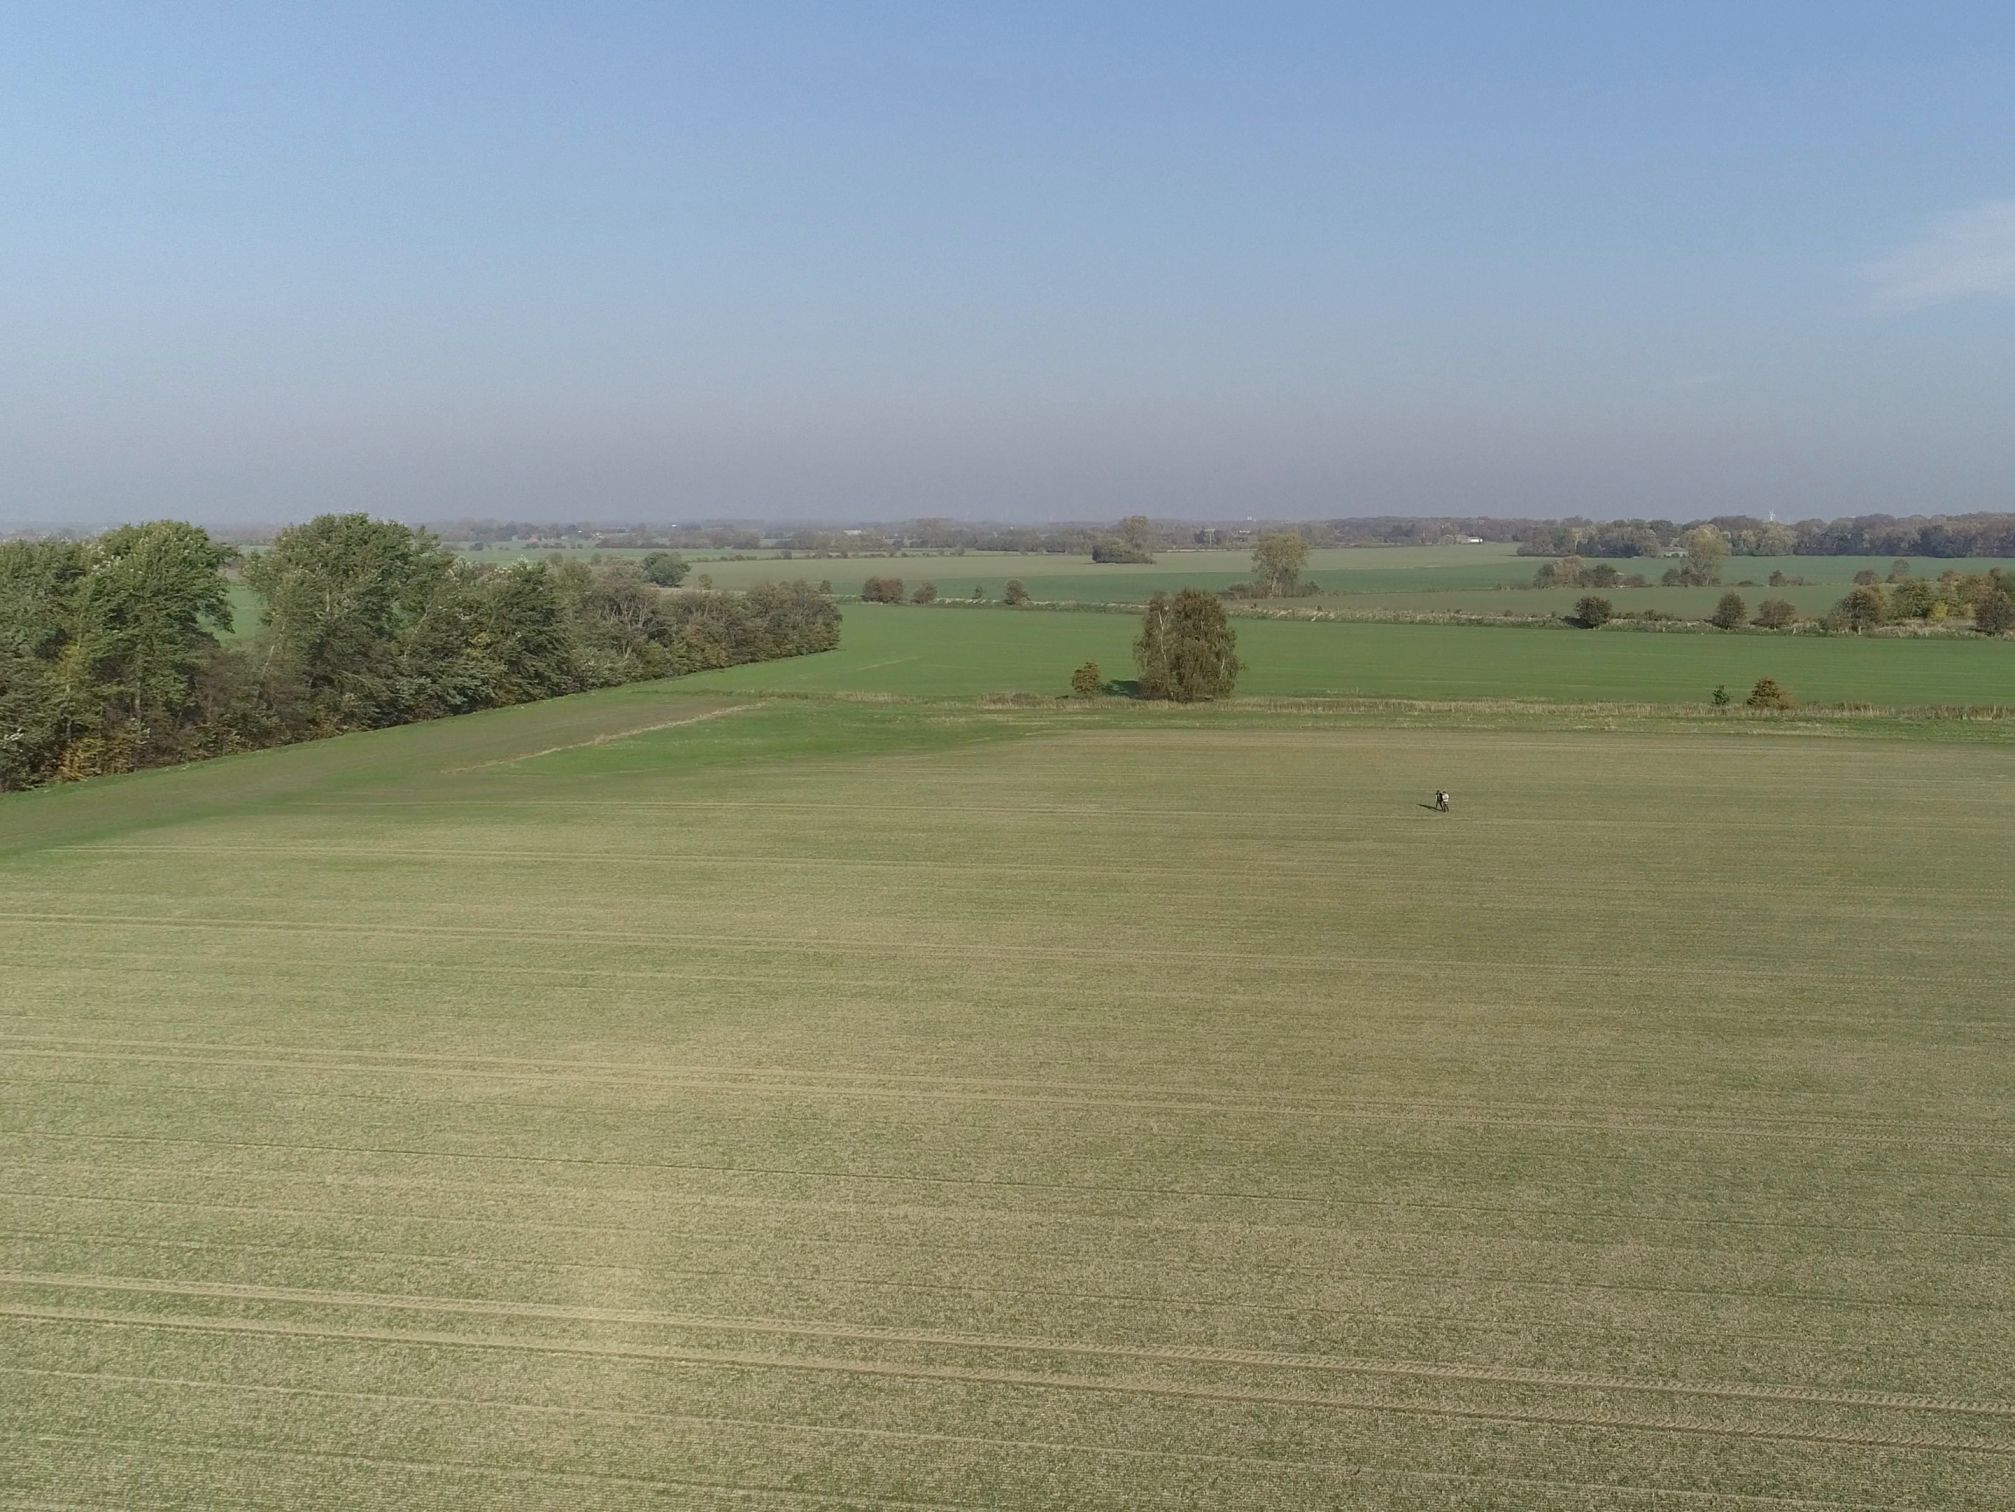
\includegraphics[width=3.122in]{figures/source/out30(1)}};

\path[fill=foo,line join=round,fill opacity=0.35,line width=0.256pt] (0.0000,247.7590) -- (227.8430,146.1690) -- (403.2000,150.1500) -- (403.2000,273.8490) -- (0.0000,247.7590) -- cycle;

\path[draw=white,line join=round,line width=0.512pt] (19.6911,244.5640) -- (56.0711,227.9040);



\path[draw=white,line join=round,line width=0.512pt] (19.8503,205.9030) -- (19.8504,244.6440) -- (67.5301,247.1570);



\path[fill=white,line join=round,line width=0.160pt] (63.6000,244.7010) -- (65.5307,247.0370) -- (63.4689,249.0560) -- (69.3046,247.0560) -- (63.6000,244.7010) -- cycle;



\path[fill=white,line join=round,line width=0.160pt] (52.5130,227.1350) -- (55.3596,228.1760) -- (54.6000,230.9590) -- (58.6260,226.2860) -- (52.5130,227.1350) -- cycle;



\path[fill=white,line join=round,line width=0.160pt] (17.6441,209.5580) -- (19.8958,207.5300) -- (22.0002,209.5030) -- (19.7535,203.7580) -- (17.6441,209.5580) -- cycle;



\path[cm={{1.0,0.0,0.0,1.0,(13.0,267.0)}}] (0.0000,0.0000) node[above right] () {\color{white}$\mathcal{O}_W$};



\path[cm={{1.0,0.0,0.0,1.0,(69.0,259.0)}}] (0.0000,0.0000) node[above right] () {\color{white}$x$};



\path[cm={{1.0,0.0,0.0,1.0,(50.0,220.0)}}] (0.0000,0.0000) node[above right] () {\color{white}$y$};



\path[cm={{1.0,0.0,0.0,1.0,(10.0,203.0)}}] (0.0000,0.0000) node[above right] () {\color{white}$z$};

\end{tikzpicture}


  \caption[The covering problem in a precision agriculture scenario]{The covering problem in a precision agriculture scenario. The aerial robot has to cover an agricultural field that forms a polygon (blue/transparent area in the frame) and run some autonomous tasks {\scriptsize(photo credit: Amit Ferencz Appel)}.}
  \label{fig:plot2}
\end{figure}

In the remainder of this work, we refer to computational tasks that can be scheduled in an energy-aware fashion as computations, opposed to the other tasks with no significant effect on energy consumption. We assume the aerial robot runs the computations on the heterogeneous computing hardware. As an example, we refer to an aerial robot in a precision agriculture scenario in \fref{fig:opterra}{Figure}, which covers an agricultural field. 
\begin{figure}[h]
  \centering
  
\def \globalscale {1.00000}
\begin{tikzpicture}[y=0.80pt, x=0.80pt, yscale=-.7*\globalscale, xscale=.7*\globalscale, inner sep=0pt, outer sep=0pt,spy using outlines={circle,white,magnification=12,size=2cm, connect spies}]

\path[cm={{1.0,0.0,0.0,1.0,(0,0)}}] (0.0000,0.0000) node[below right] () {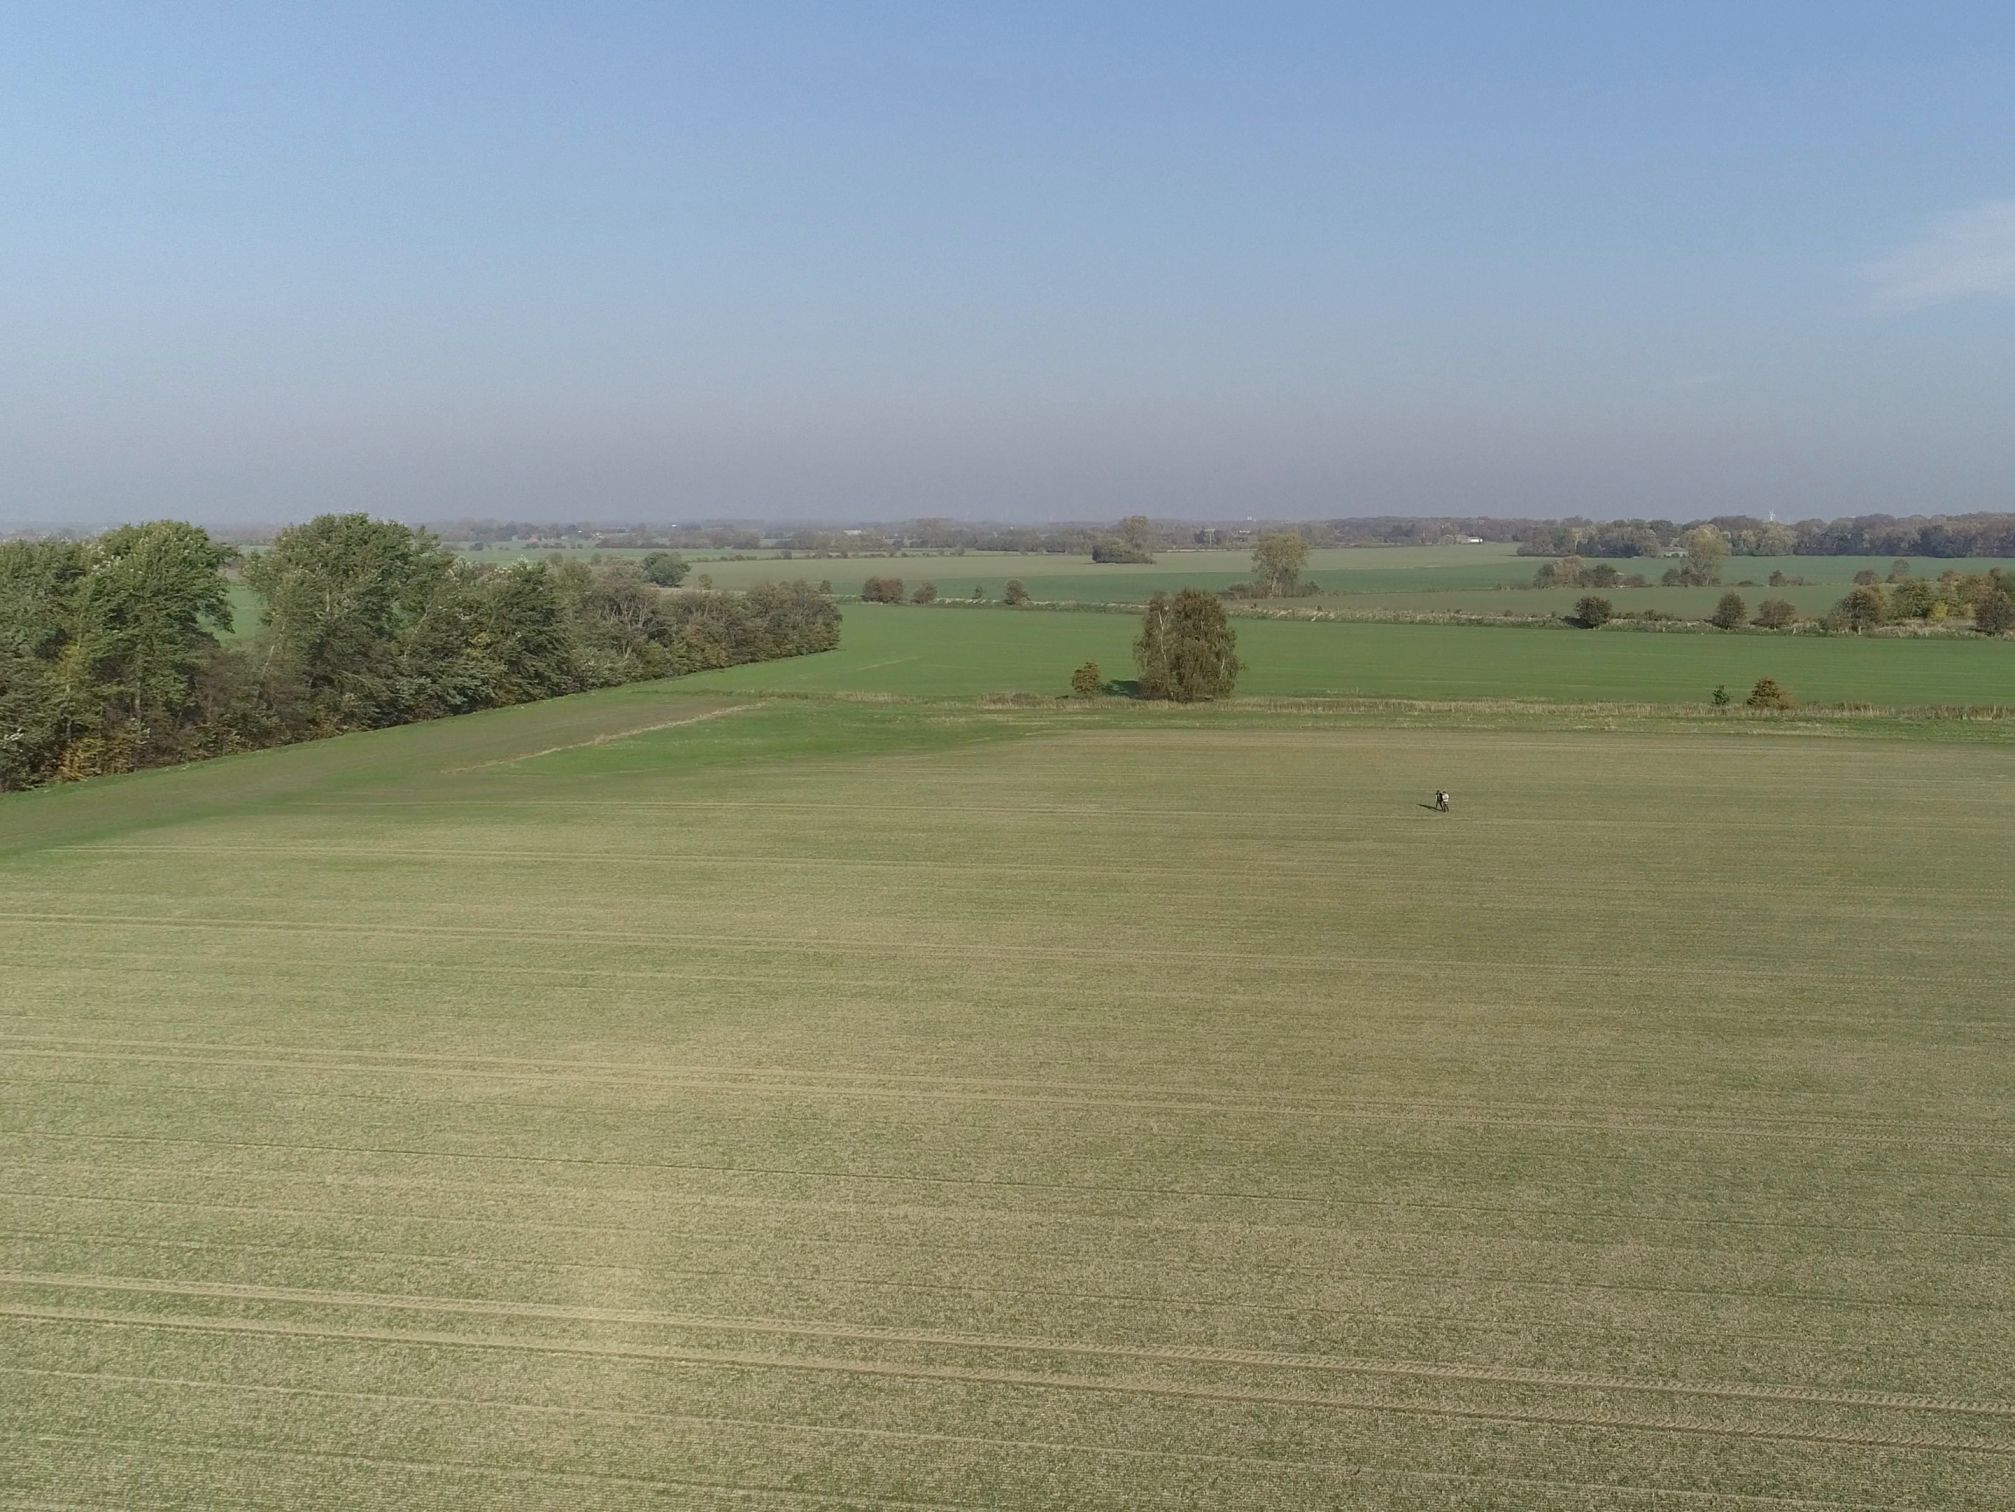
\includegraphics[width=3.122in]{figures/source/out30(1)}};


\spy on (201.6,-112) in node [left] at (160,100);

\end{tikzpicture}


  \caption[The hazard detection in the precision agriculture scenario]{The aerial robot detects hazard on the agricultural field and communicate the detection to ground-based actors while it cover the polygon.}
  \label{fig:plot2x}
\end{figure}
In abstract terms, the field is represented by a polygon in \fref{fig:plot2}{Figure} and the aerial robot detects some patterns on such polygon using a convolutional neural network (\Gls{acr:cnn})\findex{convolutional neural network} in \fref{fig:plot2x}{Figure}. The aerial robot further communicates the position of a detected pattern to other, ground-based actors. Detecting the patterns usually involves heterogeneous computing elements (GPU\findex{GPU} and/or multiple CPU\findex{CPU} cores) and consumes a significant amount of energy as opposed to communication. Detection is a computation, while communication is an (energy-inexpensive) task.

We are interested in the energy optimization of the path and computations under uncertainty (atmospheric interferences) in-flight and refer to it as dynamic energy planning. Unlike most of the past mobile robotics planning literature, the approach that we propose plans these two aspects simultaneously. Such planning would find optimal tradeoffs\findex{tradeoffs} between the path, computations, and energy requirements. Current generic planning solutions for aerial robots do not plan the path and computations dynamically, nor are they energy-aware. They are often semi-autonomous: the path and computations are static and usually defined using planning software~\citep{daponte2019review}. Instances of the planning software include famous flight controllers~\citep{px4,papa}. Such a state of practice has prompted us to investigate the topics presented in this work. We will gradually propose a dynamic energy planning approach for aerial robots. It plans both the path and computations while the aerial robot is flying and its batteries draining. 

%!
We formally define the robot planning problem after outlining the approach in the next section.


%%%%%%%%%%%%%%%%%%%%%%%%%%%%%%%%%
\section{Outline of the Approach}
\label{sec:outline}

In this work, we address the increasing demands for autonomy of modern aerial robots with a dynamic planning approach. The approach provides a simultaneous energy-aware plan of the path and a power-saving schedule of the computations. To this end, we first need a user-defined initial plan that is then replanned energy-wise using an energy model for future prediction. Later, an algorithm inputs the initial plan, estimates the state of the energy model, evaluates future energy consumption and replans parameters relative to the path and computations. The plan consists of different stages. At each stage, the aerial robot flies a path and executes some computations. Furthermore, it contains some additional parameters to alter the path and computations along with an energy budget. The alterations are bounded. There are path constraint sets that bound the path alterations and computations constraint sets, one per each computation, that bound computations alterations.

We use the concept of different stages to model complex paths. For instance, the path might contain multiple circles and lines. We will see such plan later in \fref{sec:flight-plan}{Section}. The approach guides the aerial robot on different paths (the plan is composed of) using vector field~\citep{de2017guidance}. The robot switches between the paths as soon as it reaches specific triggering points. 

The approach further relies on \powprof{}, a profiling and modeling tool that we introduce in \fref{sec:comp-ener-model}{Section}. The tool models the energy consumption of the computations and is later employed to estimate the future energy of the aerial robot in flight. To this end, we empirically derive and formally prove a periodic energy model that accounts for the uncertainty. We use Fourier analysis to derive the model and state estimation to address the uncertainty. Periodicity is often present due to repetitive patterns in the plan~\citep{seewald2020mechanical}. Indeed, mobile robots often iterate over a set of tasks and paths~\citep{seewald2021energy}. Given that the plan is periodic, we expect the energy consumption to evolve (approximately) periodically. We describe in detail such model in \fref{sec:periodic-model}{Section}. 

The replanning of the path and computations is achieved with modern optimal control techniques, such as optimal state estimation in \fref{cp:est}{Chapter}, and  model predictive control (MPC)~\citep{rawlings2017model} in \fref{cp:opt}{Chapter}. The control is data-driven. Energy sensor data estimates some coefficients of the model used to predict the future energy consumption with uncertainty. The replanning is done under an energy budget--the battery capacity and other battery parameters. Our goal is to complete the plan with the highest possible parameters configuration. 


%%%%%%%%%%%%%%%%%%%%%%
\section{Applications}

The dynamic energy planning in this work applies to modern aerial robots with a certain degree of autonomy. By the latter, we mean that the robot performs at least a predefined set of tasks over a given space. Although most of the guidance in \fref{cp:gd}{Chapter} is designed for aerial robots specifically, the approach can be easily adapted to other mobile robots with energy constraints. We discuss applications out of aerial robotics domain further in \fref{cp:conc}{Chapter}. For instance, we have applied the approach to the space robotics context~\citep{seewald2020beyond}. 

In the remainder of this work, we focus on the precision agriculture scenario in \fref{fig:plot2}{Figure}. In summary, the aerial robot covers a given agricultural field (a polygon) and searches for ground hazards. With the scenario, we validated the work experimentally. Path-wise, the aerial robot flies in circles and lines covering the polygon. Computation-wise, it detects hazards using the CNN and notifies grounded mobile robots employed for, e.g., harvesting. The approach alters the plan; it controls the processing rate and the radius of the circles affecting the distance between the lines. We will see this concrete scenario described formally in \fref{sec:flight-plan}{Section} and solved progressively in the remaining chapters.

%We observe that not only the path but also the computations significantly impact the energy, with a potential extension of up to 13 minutes over an hour by switching from the highest to the lowest level of computations in presence of a standard battery.


%%%%%%%%%%%%%%%%%%%%%%%%%%%%%%%%%
\section{Contribution}

With this work, we contribute with a dynamic planning approach for aerial robots performing autonomous scenarios for different use-cases, under energy constraint, and in an uncertain environment. In particular, we plan both an energy-optimized path and a power-saving schedule. Indeed dynamic planning that incorporates both these aspects simultaneously is underrepresented in the literature. 

The contribution in this work builds upon some other past contributions. In particular, our computational energy modeling relies on an automated profiling and modeling methodology that we proposed in~\citep{seewald2019coarse}. The methodology is based on the \powprof{} tool to derive an energy model for future energy prediction. We proposed an extension of \powprof{} with a component-based energy modeling approach to abstract per-component energy in a dataflow computational network in~\citep{seewald2019component}. We later integrated the tool in a Robot Operating System (ROS)~\citep{quigley2009ros} in~\citep{zamanakos2020energy}.

The agricultural scenario that we briefly introduced in \fref{sec:objective}{Section} is based on simulation of detections over a field under varying atmospheric conditions and with different scheduling options that we proposed in~\citep{zamanakos2020energy}, the energy modeling approach on some empirical observations. We proposed a periodic energy modeling in~\citep{seewald2020mechanical} using the empirical energy data of the Opterra aerial robot flying the precision agriculture scenario. 

A dynamic planning approach that we proposed in~\citep{seewald202Xenergy} relies on all the concepts that we propose in this work and derives simultaneously the energy-optimized path and the power-saving schedule. Additionally to dynamic planning for aerial robots, we studied the approach on different robots in~\citep{seewald2020beyond}.


%%%%%%%%%%%%%%%%%%%
\section{Structure}
\label{sec:structure}

\begin{figure}[!h]
  \centering
  \hspace*{-6ex}
  \footnotesize\fontfamily{phv}\selectfont
  \begin{tikzpicture}[auto, node distance=3cm,>=latex']
      \node [block,node distance=1cm] (theblock0) {Introduction,~\fref{cp:intro}{Ch.}};
      \node [block,below=1cm,node distance=1cm] (theblock) {Planning Problem,~\fref{cp:pb}{Ch.}};
      \node [block,below=5.5cm] (theblock2) {Optimal Control Generation,~\fref{cp:opt}{Ch.}};
      \node [block,below left=1cm and -.6cm of theblock] (theblock3) {Energy Models,~\fref{cp:model}{Ch.}};
      \node [block,below right=.5cm and 2.3cm of theblock3] (theblock4) {Guidance,~\fref{cp:gd}{Ch.}};
      \node [block,below=.5cm and -.5cm of theblock3] (theblock5) {State Estimation,~\fref{cp:est}{Ch.}};
      \draw [->] (theblock0) -- node{} (theblock);
      \draw [->] (theblock) -- node{} (theblock2);
      \draw [->] (theblock5) |- node{} (theblock2);
      \draw [->] (theblock2) -| node{} (theblock4);
      \draw [->] (theblock5) -- node{} (theblock3);
      \draw [->] (theblock) |- node{} (theblock3);
      \draw [->] (theblock) |-   node{} (theblock4);
      \draw [decorate,decoration={brace,amplitude=10pt,mirror,raise=64pt},yshift=0pt]
      (theblock5.north west) -- (theblock5.north west -| theblock4.north east) node [black,midway,yshift=-25ex] (notextnode) {};
      \node [block,below=-.8cm and -.5cm of notextnode,xshift=-3.3cm] (theblock6) {Implementation,~\fref{app:imp}{App.}};
      \node [block,below=-.8cm and -.5cm of notextnode,xshift=1.1cm] (theblock8) {Summary and Future Directions,~\fref{cp:conc}{Ch.}};
      \node [below=-.4cm and -.5cm of notextnode,xshift=-1.62cm] (comma) {,};
      \node [block,left of=theblock3,node distance=3cm,yshift=1.15cm] (theblock7) {State of the Art,~\fref{cp:soa}{Ch.}};
      \draw [->] (theblock7) |- node{} (theblock);
      \draw [->] (theblock7) |- node{} (theblock3);
      \draw [->] (theblock7) |- node{} (theblock2);
  \end{tikzpicture}
  \caption[Diagram of the structure]{Diagram of the structure of this work. The arrows are to be read with ``the chapter influences'' in the direction of the arrow. \fref{cp:intro}{Chapter} serves as an introduction while \fref{cp:soa}{Chapter} presents the state of the art. \fref{cp:pb}{Chapter} presents the planning problem, which is solved in \fref{cp:opt}{Chapter} using notions from \fref{cp:model}{Chapters}\fref{cp:est}{--\hspace*{-.8ex}}. \fref{cp:est}{Chapter} presents the guidance action to move over a replanned. \fref{cp:conc}{Chapter} concludes the work and proposes future directions and \fref{app:imp}{Appendix} the implementation.}
  \label{fig:structure}
\end{figure}

The remainder of this work is illustrated in \fref{fig:structure}{Figure} structured as follows. In this chapter, we introduced the dynamic energy planning for aerial robots. We define the planning problem in \fref{cp:pb}{Chapter}, and propose the solution to the problem in \fref{cp:opt}{Chapter}, which builds upon the topics presented in the remaining chapters. In particular, in \fref{cp:soa}{Chapter} we present the state-of-the-art in energy modeling and planning for mobile robots. We include some energy models for heterogeneous computing hardware.

Dynamic planning requires accurate future energy predictions. We present the derivation of some energy models to address future energy predictions in \fref{cp:model}{Chapter}. Specifically, we propose energy models for computations, motion, and the battery. We derive and formally prove a periodic energy model that we use in the remainder of this work to predict future energy consumption. The periodic energy model's accuracy depends on the availability of measurements of energy data. We detail the process in \fref{cp:est}{Chapter}. We describe how to estimate the coefficients of the periodic energy model and refine the future predictions with the available data.

Flying on a dynamic plan requires the derivation of a guidance action to guide the aerial robot in space. This process is elaborated in \fref{cp:gd}{Chapter}. We discuss an approach to guide the aerial robot in space on the planned path. 

An optimal solution for the dynamic mobile robot planning problem relies on optimal control techniques. We describe such techniques in \fref{cp:opt}{Chapter}. Specifically, after summarizing some of these techniques, we propose an optimization algorithm to select the optimal parameters configuration for the path and computations simultaneously. Finally, we conclude our work in \fref{cp:conc}{Chapter} along some recommendations for future research direction. 

We then present some additional information in appendices. In \fref{app:imp}{Appendix} we propose the implementation in MATLAB(R) of the planning problem, the model, the estimation technique, the guidance action, and the derivation of the optimal control. 

